% SPDX-License-Identifier: CC-BY-SA-4.0
%
% Copyright (C) 2026 embedded brains GmbH & Co. KG
\documentclass[tikz,border=4pt]{standalone}
\usepackage[T1]{fontenc}
\usepackage[scaled]{helvet}
\renewcommand{\familydefault}{\sfdefault}
\usetikzlibrary{arrows.meta,backgrounds,positioning,calc,fit,automata}
\definecolor{ebblue}{HTML}{1F4E79}
\definecolor{boxfill}{HTML}{EAF1F8}
\definecolor{codefill}{HTML}{FFF4E0}
\definecolor{codeline}{HTML}{9C6500}
\definecolor{groupfill}{HTML}{F5F5F5}
\definecolor{flow}{HTML}{404040}
\definecolor{earsfill}{HTML}{E8F4E8}
\definecolor{earsline}{HTML}{2E7D32}
\begin{document}
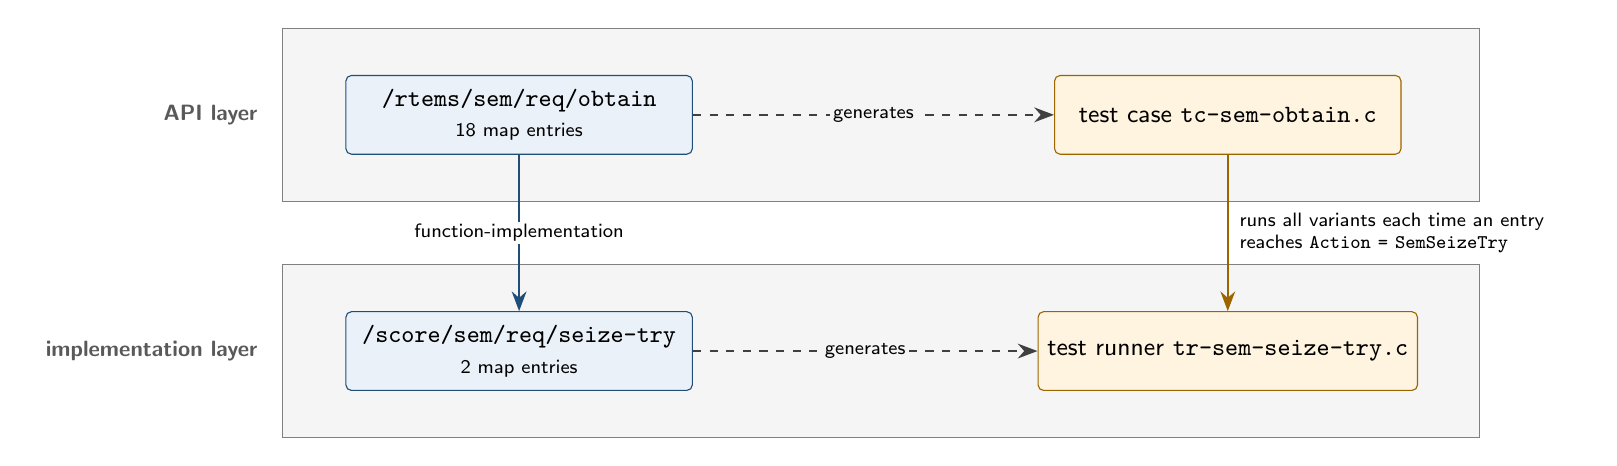
\begin{tikzpicture}[
    font=\small,
    req/.style={draw=ebblue, fill=boxfill, rounded corners=2pt,
      minimum width=44mm, minimum height=10mm, align=center},
    test/.style={draw=codeline, fill=codefill, rounded corners=2pt,
      minimum width=44mm, minimum height=10mm, align=center},
    gen/.style={-{Stealth[length=2.5mm]}, thick, dashed, draw=flow},
    run/.style={-{Stealth[length=2.5mm]}, thick, draw=codeline},
    impl/.style={-{Stealth[length=2.5mm]}, thick, draw=ebblue},
    lbl/.style={font=\scriptsize, align=center, fill=groupfill, inner sep=1pt},
    lanelabel/.style={font=\footnotesize\bfseries, text=gray!70!black,
      align=right, anchor=east, text width=28mm}]
  \foreach \y/\name in {3/API layer, 0/implementation layer} {
    \fill[groupfill] (-2.6,\y-1.1) rectangle (12.6,\y+1.1);
    \draw[gray] (-2.6,\y-1.1) rectangle (12.6,\y+1.1);
    \node[lanelabel] at (-2.8,\y) {\name};
  }
  \node[req] (obtain) at (0.4,3) {\texttt{/rtems/sem/req/obtain}\\\scriptsize 18 map entries};
  \node[req] (try) at (0.4,0) {\texttt{/score/sem/req/seize-try}\\\scriptsize 2 map entries};
  \node[test] (tc) at (9.4,3) {test case \texttt{tc-sem-obtain.c}};
  \node[test] (tr) at (9.4,0) {test runner \texttt{tr-sem-seize-try.c}};
  \draw[impl] (obtain) -- node[lbl, fill=white] {function-implementation} (try);
  \draw[gen] (obtain) -- node[lbl] {generates} (tc);
  \draw[gen] (try) -- node[lbl] {generates} (tr);
  \draw[run] (tc) -- node[lbl, right=1mm, align=left, fill=none, text width=44mm]
    {runs all variants each time an entry\\reaches \texttt{Action = SemSeizeTry}} (tr);
\end{tikzpicture}
\end{document}
